\chapter{Elemente ale arhitecturii software}
\label{chap:soft}

\section{Achizi\c{t}ie date \c{s}i constr\^{a}ngeri de timp} \label{time}

Una dintre caracteristicile principale ale unui sistem în timp real este faptul că acesta trebuie să răspundă schimbărilor venite din mediul înconjurător în limita unui interval de timp, numit \emph{deadline} \cite{str}. Pentru funcționarea corespunzătoare a sistemului, sunt necesare date din 2 surse diferite: senzorii ce detectează prezența unui obiect și senzorul de luminozitate. 

În cazul senzorilor de prezență, este important ca intervalul de timp dintre 2 citiri să fie mai mic decât cel necesar trecerii în întregime a unui vehicul prin fața acestuia. Dacă aș considera suprafața în care senzorii detectează un obiect a fi de lățime neglijabilă,  pot afla viteza necesară pentru ca vehiculul să treacă nedetectat. În crearea programului Arduino după care funcționează sistemul, am observat faptul că intervalul de timp dintre două citiri ale aceluiași senzor este de 15-17 ms (puțin peste 1 tick). 

În exemplul ilustrat în \figref{fig:car4}, am analizat cazul extrem al unei motociclete de lungime relativ mică, 190cm. La convertirea din cm/ms în km/h a rezultat faptul că aceasta ar trebui să atingă o viteză de aproximativ 402km/h pentru a depăși un senzor complet nedetectată.  Prin urmare, frecvența citirilor este suficient de mare pentru a acomoda cerințele sistemului real, și chiar pentru a permite unele modificări aduse cu scopul de a îmbunătăți performanțele sau de a adăuga utilități extra. 

\begin{figure}[!ht]
    \begin{center}
    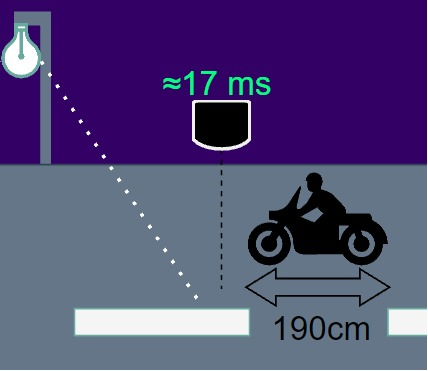
\includegraphics[width=0.5\linewidth,keepaspectratio]{pics/cardraw4.jpg}
    \end{center}
    \caption{Timp citire date}
    \label{fig:car4}
\end{figure}
 Pentru lumină, nu contează atât de mult cât de des se realizează achiziția de date de la senzor, deoarece valoarea citită oricum variază lent. Totuși, și aceasta se va citi la fiecare repetare a task-ului dedicat ei, deoarece trebuie să țină pasul cu citirile senzorilor. Motivul pentru acest fapt este prezentat mai detaliat în \ref{light}.

\section{Descriere FreeRTOS}
Pentru a îndeplini cerințele sistemului în timp real pe care l-am simulat, și aplicația ce determină funcționarea acestuia trebuie să poată folosi concepte specifice programării în timp real \cite{patr}. Este necesară utilizarea firelor de execuție și a semafoarelor pentru a asigura funcționarea în conformitate cu performanțele dorite. De aceea folosirea unui \gls{rtos} este obligatorie. Deși aceasta nu este o caracteristică de bază a Arduino IDE, includerea bibliotecii FreeRTOS permite utilizarea funcțiilor necesare creării și gestiunii firelor de execuție(sub formă de task-uri), a semafoarelor și a mutex-urilor. Această bibliotecă deschide accesul și la funcția vTaskDelay, ce oferă posibilitatea blocării unui anumit task, fără afectarea celorlalte task-uri. Poate fi apelată pentru o durată de timp specificată ori în număr de ticks, ori în milisecunde, prin conversie.

\section{Prezentare task-uri} \label{task}
 În cadrul aplicației am folosit 3 task-uri, ce funcționează după secvența logică din \figref{fig:diag_task-uri}. Ele au aceeași prioritate și se execută în același timp. Ordinea efectuării operațiilor din fiecare task, relativ la celelalte task-uri, este influențată prin incrementarea și decrementarea semafoarelor, unde este necesar.


\begin{figure}[!ht]
    \begin{center}
    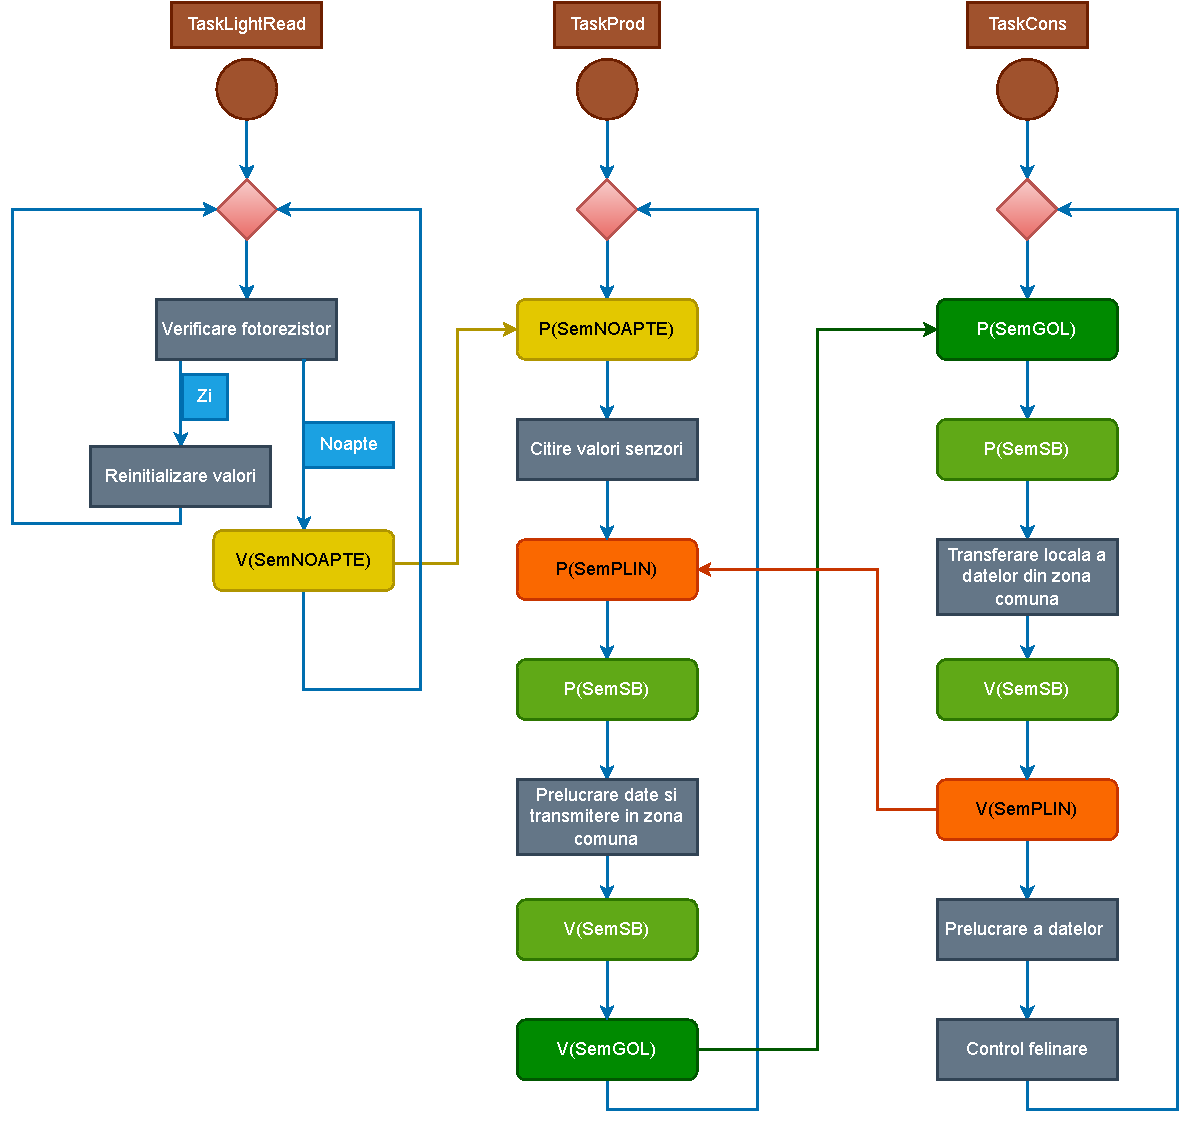
\includegraphics[width=0.9\linewidth,keepaspectratio]{pics/diag.drawio.pdf}
    \end{center}
    \caption{Diagramă task-uri}
    \label{fig:diag_task-uri}
\end{figure}

\subsection{TaskLightRead} \label{light}
 În task-ul acesta (\ref{tlr}) se realizează citirea intrării analogice de pe pin-ul plăcii Arduino la care este conectat fotorezistorul. Dacă valoarea acesteia depășește o anumită constantă, se consideră că afară este zi, urmând reinițializarea tuturor variabilelor folosite la valori nule, pentru a nu rămâne cu cele obținute anterior. Dacă felinarele erau aprinse, sau pe modul de intensitate scăzuta, aici se sting \textbf{complet}. În cazul în care valoarea citită este sub limita impusă, se incrementează semaforul binar SemNOAPTE, cu scopul de a debloca TaskProd.

 Deși acesta este modul normal de funcționare al task-ului, în codul sursă (\ref{tlr}) al aplicației realizate de mine verificarea are loc invers: deblocarea celorlalte două task-uri se întâmplă doar pe timp de zi, pentru ușurarea procesului de testare.
\subsection{TaskProd}
 Acest task producător (\ref{tp}) are rolul de a citi valorile de la senzorii de prezență, lucru care se întâmplă imediat după deblocarea sa, în urma incrementării semaforului SemNOAPTE. Mai departe, la prima rulare, se decrementează semaforul binar SemPLIN, dar se trece, totuși, mai departe, deoarece acesta este inițializat cu valoarea "1". Același lucru este valabil și pentru semaforul pentru secțiunea critică, SemSB, care asigură faptul că zona comună de date nu este accesată simultan de mai multe task-uri \cite{patr}. În urma alterării și transferării noilor date, acesta este deblocat. Apoi, semaforul binar SemGOL este incrementat, pentru deblocarea task-ului TaskCons. La rulări ulterioare ale task-ului, acesta se va bloca fie în SemNOAPTE, dacă s-a făcut zi, sau în SemPLIN, dacă nu a fost incrementat din TaskCons. 
\subsection{TaskCons}
 Deblocarea task-ului consumator (\ref{tc}) are loc la incrementarea în TaskProd a semaforului SemGOL. Urmează trecerea datelor din zona comună în plan local, facilitată de semaforul SemSB. În urma incrementării lui SemPLIN, ce permite deblocarea lui TaskProd, are loc prelucrarea datelor obținute și controlul felinarelor conform condițiilor impuse. În final, task-ul se repetă, în concordanță cu toate cele menționate pană acum.
\section{Analiz\u{a} a codului}

 În această secțiune voi menționa și descrie câteva fragmente mai importante din codul sursă, cu scopul de a oferi o privire mai clară asupra modului de funcționare al aplicației. Toate variabilele scalare sau vectoriale vor fi inițializate în întregime cu 0, cu excepția unora dintre semafoare, conform Secțiunii \ref{task}. Constanta $d$ reprezintă distanța (în cm) dintre 2 senzori consecutivi și este egală cu 14. În cazul buclelor for, acestea în general se repetă de $n = 5$ ori dacă sunt folosite valorile corespondente senzorilor de prezență, sau de $n - 1 = 4$ ori, pentru operații ce influențează calculul sau afișarea vitezei pe o anumită porțiune de drum.

\subsection{Prelucrare date citite și counter obiecte} \label{counter}
\indent \indent 
Modulele cu senzor infraroșu folosite pot avea ca ieșiri valorile "1", când nu se află nimic în fața lor, sau "0", când au un obiect în față. Aceste valori numerice nu ajută foarte mult, deoarece scopul  este de a obține viteza vehiculului. De aceea va fi utilizată funcția millis() din Arduino IDE, pentru a obține  timpul (în ms) trecut de la momentul rulării aplicației până la activarea unui senzor.

În următorul fragment de cod este prezentată zona de \emph{Prelucrare date și transmitere în zona comună} din TaskProd. În aplicația realizată de mine, drumul este împărțit în n-1 porțiuni egale ca dimensiune, aflate între cei n senzori de prezență folosiți.

\begin{verbnobox}[\verbarg]
     for(int in = 0; in < 5; in ++){
        if (f[in] == 1){
          b[in]= bn[in];
          bn[in] = 0;
          f[in] = 2;
        }
        if (aux[in] - bc[in] == 1) {
            if (in <= 3) {
              c[in] ++;
            }
            if ((in >= 1) && c[in-1]>0){
              c[in - 1] --;
             if ((bn[in-1] != 0) &&(c[in - 1] == 1)){
                  f[in-1] = 1;
               } 
           }      
            if (in == 4)
              b[in] = millis();
            else if ((in <= 3) && (c[in] == 1)){ 
                  b[in] = millis();
            }
            else if ((in <= 3) && (c[in] > 1)){
                bn[in] = millis();
            }
         }
          aux[in] = bc[in];      
      }   
\end{verbnobox}

Numărul de vehicule de pe fiecare porțiune de drum este salvat în vectorul counter $\mathbf{c[n - 1]}$, iar acesta este actualizat la fiecare depășire a unuia dintre senzori de un vehicul. Este important ca atât modificarea valorii din $\mathbf{c}$, cât și cea a momentului de timp înregistrat, să se întâmple o singură dată la fiecare activare a unui senzor de prezență. Pentru a îndeplini această cerință cu acuratețe, trebuie recunoscute doar momentele când un obiect apare în fața unui senzor, sau, mai precis, când valoarea citită de la senzor se transformă din "1" în "0". Vectorul $\mathbf{bc[n]}$ conține valorile obținute în secțiunea de Citire valori senzori, iar egalarea elementelor din $\mathbf{aux[n]}$ la finalul buclei for face ca la următoarea execuție a task-ului să pot compara valoarea actuală cu cea citită cu un pas în urmă. Diferența dintre cele două poate fi egală cu 1 doar în cazul dorit, cel în care $\mathbf{aux[in]}=1$ și $\mathbf{b[in]}=0$. În cazul unui singur vehicul,  momentul la care a fost activat un senzor este salvat în $\mathbf{b[n]}$. Am adăugat variabilele vectoriale $\mathbf{f[n]}$ și $\mathbf{bn[n]}$, pentru tratarea cazului în care mai multe vehicule se află pe aceeași porțiune de drum. Un exemplu al unei astfel de situații este reprezentat în \figref{fig:doi1} și \figref{fig:doi2} .
\begin{figure}[!ht]
    \begin{center}
    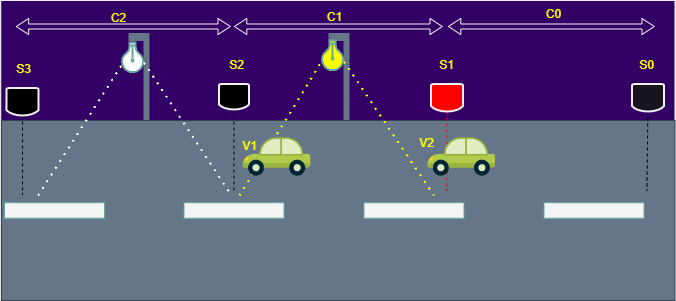
\includegraphics[width=0.7\linewidth,keepaspectratio]{pics/doi1.png}
    \end{center}
    \caption{Situație 2 vehicule pe aceeași porțiune de drum, moment 1}
    \label{fig:doi1}
\end{figure}

\begin{figure}[!ht]
    \begin{center}
    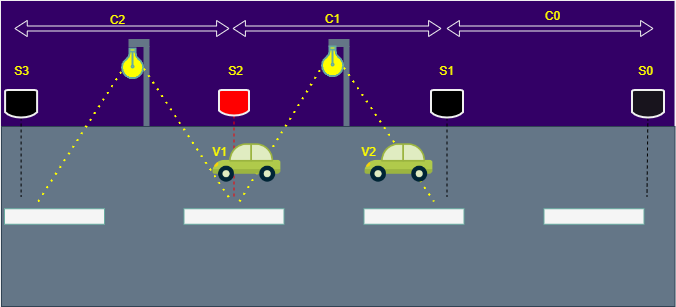
\includegraphics[width=0.7\linewidth,keepaspectratio]{pics/doi2.png}
    \end{center}
    \caption{Situație 2 vehicule pe aceeași porțiune de drum, moment 2}
    \label{fig:doi2}
\end{figure}

În această situație, comportamentul aplicației pe porțiunea de cod descrisă este următorul:
\begin{enumerate}
\item  La depășirea senzorului S1 de vehiculul V2, counter-ul $\mathbf{c[1]}$ este incrementat și are valoarea 2. Momentul de timp este salvat în vectorul $\mathbf{bn[1]}$.
\item  La activarea lui S2, momentul este salvat în $\mathbf{b[2]}$, iar flag-ul $\mathbf{f[1]}$ primește valoarea 1.
\item  La următoarea execuție a task-ului, acest flag indică faptul că valoarea din $\mathbf{b[1]}$ nu mai este necesară, deoarece a fost folosită deja în calculul unei viteze. Ea va fi înlocuită cu valoarea din $\mathbf{bn[1]}$, iar $\mathbf{f[1]}$ va deveni 2. În această stare, el indică faptul că următorul calcul al vitezei cu noul $\mathbf{b[1]}$ este doar unul intermediar și nu va influența luminozitatea felinarelor.   

\end{enumerate}

Această metodă de implementare acoperă și cazul apariției unui vehicul V3 în porțiunea C1, înaintea ieșirii lui V2 din aceasta, prin eliberarea lui $\mathbf{bn[1]}$ pentru trecerea lui V3 prin S1. Modelul realizat funcționează doar până la limita de 2 vehicule existente simultan în aceeași porțiune. Pentru generalizare, vectorul $\mathbf{bn}$ ar trebui să fie o matrice de $n$ coloane și $m$ linii, unde $m$ este un număr natural, cu 1 mai mic decât numărul de automobile maxime admise într-o porțiune a drumului, ales în funcție de lungimea porțiunii respective.


\subsection{Transmitere date între task-uri}
 Pentru folosirea datelor primite de la senzorii de prezență, este necesar transferul între task-uri prin folosirea unor vectori declarați global, astfel:

\begin{verbnobox}[\verbarg]
for (int i = 0; i < 5; i ++) { 
      z[i] = b[i];
      zn[i] = bn[i];
    }
\end{verbnobox}


\subsection{Transformare date senzori mișcare în valori de timp \c{s}i \^{i}n vitez\u{a}}
Pentru aflarea vitezei, se scad momentele de timp la care au fost activați 2 senzori consecutivi și se realizează transformarea prin calcule matematice, în funcție de unitatea de măsură dorită că rezultat. În cazul meu, conversia este din cm/ms în km/h. Diferențierea între valorile lui $\mathbf{c}$ ale secțiunii în care intră vehiculul se face pentru a determina dacă valoarea de timp corespondentă acestuia trebuie luată din $\mathbf{z}$ sau $\mathbf{zn}$. Deși viteza este calculată la fiecare rulare a task-ului în $\mathbf{vint[n-1]}$vint, aceasta este salvată în $\mathbf{v[n-1]}$ și afișată doar la momentul activării unui senzor, numai în situațiile în care flag-ul $\mathbf{f}$ nu este egal cu 2. Dacă acesta este 2, va fi reinițializat cu 0. În $\mathbf{auxv[n-1]}$ este salvată valoarea vitezei intermediare la execuția anterioară a task-ului, pentru comparare cu cea actuală, similar cu $\mathbf{aux}$ în \autoref{counter}.

\begin{verbnobox}[\verbarg]
for (int i = 0; i < 4; i ++) {
      if (i==3)
        t[i] = z[i + 1] - z[i];
      else if (c[i + 1] == 1)
        t[i] = z[i + 1] - z[i];
      else if (c[i + 1] == 2)
        t[i] = zn[i + 1] - z[i];
      
      if (t[i] != 0)
        vint[i] = 10*d * 3.6/((float)t[i]);
      else if (t[i] == 0) 
        vint[i] = 0;
      if (auxv[i] != vint[i]){
        if ((f[i] != 2)&&(vint[i]>=0)){
          v[i] = vint[i];
          Serial.print ... 
        }
        else {
          Serial.print ...
          f[i] = 0;
        }
      }  
      auxv[i] = vint[i];
      ...
   }
\end{verbnobox}




\subsection{Control nivel intensitate lumină}

 Pentru controlul intensității luminii, este folosită o abordare bazată pe \gls{pwm}. Aceasta permite folosirea ieșirilor digitale corespondente LED-urilor, pe post de ieșiri analogice (\autoref{mega}), convertite din valori numerice aparținând intervalului [0,255]. Aceste valori sunt păstrate în vectorul $\mathbf{lum[n-2]}$, și sunt influențate de viteza calculată a vehiculelor, astfel:

\begin{verbnobox}[\verbarg]
    for (int i = 0; i < 4; i ++) {
      ...
      if (i > 0){ 
        if (lum[i - 1] < 3)
          lum[i - 1] = 3;
        if ((c[i] == 0) && ( lum[i - 1] > 3)) {
            if (timp == 0) {
              if (lum[i - 1] > 8)
                lum[i - 1] = lum[i - 1] * 0.7;
              else
                lum[i - 1] --;
            }
            timp ++;
            timp = timp % 5;      
        }
        else if (c[i] == 0) {     
        }
        else if (c[i] == 1){
          if (v[i-1] > 4){ 
            lum[i - 1] = 255;      
          }
          else if (v[i-1] > 1){ 
             if (lum[i - 1] > 150)
               lum[i - 1] =  lum[i - 1] - 2;
             else 
               lum[i - 1] = 150;
          }           
          else if (v[i - 1] > 0){ 
             if (lum[i - 1] > 40)
               lum[i - 1] =  lum[i - 1] - 2;
             else 
               lum[i - 1] = 40;
          }
         }
         else if (c[i] == 2){
          if ((v[i - 1] > 4)&& (lum[i - 1] < 150)){ 
            lum[i - 1] = 255;      
          }
          else if ((v[i - 1] > 1) && (lum[i - 1] < 150)){ 
            lum[i - 1] = 150;
          }           
         }  
         analogWrite(4 + i, lum[i - 1]);
        }
   }
\end{verbnobox}
 LED-urile primesc ca ieșire valoarea aflată în $\mathbf{lum}$, în cazul în care valoarea counter-ului $\mathbf{c}$ corespondent porțiunii lor de drum este diferită de 0. Când aceasta devine iar 0 (atunci când nu se mai află niciun vehicul în raza felinarului), valoarea din $\mathbf{lum}$ începe să scadă treptat, până devine 3. Valorile din $\mathbf{lum}$ se schimbă doar la modificări aduse lui $\mathbf{v}$, iar valorile din $\mathbf{vint}$ nu au niciun efect asupra lor.
 
 Diferențierea dintre cazurile în care $\mathbf{c[i]}=1$ și $\mathbf{c[i]}=2$ se face pentru a asigura faptul că este oferită o prioritate mai mare vehiculelor cu viteze mai mari, la stabilirea intensității felinarelor. Pentru momentul 1 al exemplului descris în \autoref{counter} (\figref{fig:doi1}), trecerea lui V2 prin fața lui S1 va determina schimbarea intensității luminii felinarului doar dacă viteza acestuia este mai mare decât viteza pe care a avut-o V1 la trecerea prin S1. În cazul contrar, valoarea din $\mathbf{lum}$ va începe să scadă treptat doar la ieșirea lui V1 din porțiunea C1, la momentul 2(\figref{fig:doi2}).
